% ============================================================================
%  ACM e-Energy 2027 (Winter) — full paper (acmart sigconf)
%  Title: "Staleness Makes Errors Large: Why 5-Minute Carbon-Aware Pretraining
%         Needs Fresh Signals More Than Better Forecasts"
%  Story: decision-error magnitude dominates; staleness generates the large
%  errors; the paper is decision-theoretic control + design rules + a
%  stale-aware adaptive controller. Every number traces to
%  publication/output/**/*.json.
%  Build: make   (latexmk + bibtex, acmart sigconf)
% ============================================================================
\documentclass[sigconf,nonacm=false]{acmart}

\usepackage{booktabs}
\usepackage{amsmath}
\usepackage{graphicx}
\usepackage{tikz}
\usetikzlibrary{arrows.meta, positioning}

\title{Staleness Makes Errors Large: Why 5-Minute Carbon-Aware Pretraining Needs Fresh Signals More Than Better Forecasts}

\author{Anonymous Authors}
\affiliation{%
  \institution{Anonymous Institution}
  \country{}}
\email{}

\acmConference[ACM e-Energy '27]{The 18th ACM International Conference on Future and Sustainable Energy Systems}{June 2027}{Anonymous City, Anonymous Country}
\acmYear{2027}
\acmISBN{}

\fancyhead[LO]{Staleness Makes Errors Large}
\fancyhead[RO]{Under submission to ACM e-Energy 2027}

\begin{document}

\begin{abstract}
Carbon-aware temporal shifting pauses LLM pretraining when grid carbon intensity
exceeds a threshold and resumes when it falls below. What decides whether this
works is the \emph{magnitude} of the error a decision makes: decision
\emph{staleness} generates the large errors; forecast \emph{noise} does not.
Using five years of 5-minute average carbon intensity in the three
studied grids (DE, IT, SE), we show that CI is near-unit-root (lag-1
autocorrelation $\approx0.996$; persistence $\approx$ AR(1), RMSE gap
$\le 0.06$\,g/kWh), so a stale decision is large by construction: at $h{=}72$
the persistence RMSE is $113.4$\,g/kWh (DE), $7.8\times$ a $4\sigma^*$ additive
noise, and a six-hour-stale decision costs 35.8--60.5\% of savings vs.\ $<$7\%
for that $4\sigma^*$ noise in DE and IT. At \emph{matched} magnitude additive noise is
the more damaging per unit error (DE: $2.4\%$ at 14.6\,g/kWh of noise vs.\
$0.7\%$ at 13.9\,g/kWh of staleness); staleness dominates because it generates
errors that noise does not. We formalize the \emph{grace horizon}---the maximum
staleness with $\le10\%$ loss, predicted by the empirical AR(1) $h$-step RMSE at
a level fit $k\approx0.68\cdot S$ ($R^2{=}0.91$), and propose a stale-aware
adaptive hysteresis controller that widens the margin with staleness, closing
95\%/80\% of the recoverable naive-to-oracle gap at one/three steps (DE). Under
minutes-scale checkpoints for a 671B-parameter MoE model, retention is
97.6/94.6/95.2\% at 900\,s and 91.4/85.3/81.4\% at 2700\,s. The result:
threshold design rules stable in \emph{scale} (margin scale, grace horizon)
with documented crisis-year exceptions, plus a data-freshness SLA.
\end{abstract}

\maketitle

\section{Introduction}
\label{sec:intro}

Frontier language-model pretraining has become one of the fastest-growing
single points of electricity and carbon consumption in computing
\cite{strubell2019energy,patterson2021carbon,wu2022sustainable}. A single
DeepSeek-V3-class training run consumes on the order of 2.8M GPU-hours
\cite{deepseek2024v3}, and data-center demand is projected to grow faster than
grid decarbonization \cite{maji2025crossroads}. At the same time, grids are
becoming more variable as renewables penetrate, and data centers are
increasingly expected to act as \emph{flexible} demand rather than rigid load
\cite{lin2024explodingai,lin2023adapting}. Temporal load shifting---pausing
flexible workloads when grid carbon intensity is high and resuming when it is
low---is the canonical realization of this flexibility \cite{radovanovic2022carbon,
wiesner2021letswait,dodge2022measuring}, and double-threshold pause/resume is its
provably optimal online form \cite{lechowicz2023opr}.

Every such controller faces the same pipeline: \emph{decide} on a forecast or
signal, \emph{act} by pausing/resuming training, and \emph{pay} on the emissions
that are actually realized. This paper asks a question that the carbon-aware
scheduling literature has not decomposed: at the decision scale at which such
controllers actually operate, what is the dominant source of savings loss---the
\emph{noise} of the forecast (the magnitude of the prediction error) or the
\emph{staleness} of the decision (the age of the signal on which the decision is
made)?

The two most recent anchors of this research program assume the former.
Signal-aware workload shifting with uncertainty-quantified forecasts (UQ-Advice)
treats forecast quality as the bottleneck and invests in conformal intervals to
exploit it \cite{johnson2025uqadvice}; the CI-forecasting line (CarbonCast,
EnsembleCI, CarbonX) invests in ever-better hourly ML forecasts
\cite{maji2023carboncast,yan2025ensembleci,maji2025carbonx}. At the 5-minute
decision scale we find this assumption inverted, but for a more precise reason
than ``noise is cheap'': savings loss scales with the \emph{magnitude} of the
error a decision makes, and staleness is the failure mode that \emph{generates}
large errors. Because 5-minute CI is near-unit-root, a six-hour-stale decision
carries a $113.4$\,g/kWh error in DE---$7.8\times$ a $4\sigma^*$ additive
forecast error---and costs 35.8--60.5\% of savings vs.\ $<$7\% for the
$4\sigma^*$ error itself in DE and IT; at \emph{matched} magnitude additive noise is the
more damaging per unit error. Staleness is the binding constraint because it is
the realistic source of large errors, and freshness---not forecast accuracy---is
the operational lever.

We ground this claim in five years of 5-minute average carbon intensity (ACI)
from five grids. In the three grids we study (DE, IT, SE), CI behaves like a
near-unit-root stochastic process (lag-1 autocorrelation $0.9960$--$0.9997$):
persistence and AR(1)
forecasts are statistically indistinguishable (RMSE gap $\le 0.06$\,g/kWh), and
a richer AR(7) shaves only a few g/kWh off the already-small short-horizon error.
No ML forecast of any sophistication can materially change the decision; only the
age of the signal can.

This observation has a concrete consequence for operators: the relevant design
parameter is not the forecaster but the \emph{grace horizon}---the maximum
decision staleness $h$ (in 5-minute steps) that keeps savings degradation below
10\%, predicted by the point where the empirical AR(1) $h$-step RMSE crosses
$k\approx0.68\cdot S$, $S$ the threshold-to-year-mean distance (a level fit:
$R^2{=}0.91$ over 8 region-years). The grace horizon is therefore a directly
usable data-freshness SLA: keep the decision signal fresher than $g$ steps, and
the threshold policy retains at least 90\% of its savings.

Finally, because the object of study is \emph{frontier LLM pretraining}, we
evaluate the whole scheme under realistic checkpoint economics. A 671B-parameter
MoE model has a full state of $\approx$1.34\,TB in BF16 (671e9 parameters
$\times$ 2 bytes), so checkpoint/restore is
minutes, not the 148.8\,s figure used for small models. We show that savings
survive this cost---completed-feasible retention of 81--97\% at 900--2700\,s
checkpoint times---and that the cost changes the design rules in two documented
ways: the optimized hysteresis margin must widen with checkpoint cost, and an
explicit completion constraint becomes a required design rule, because a
budget-blocked, incomplete run reports inflated savings.

Our contributions are:
\begin{itemize}
  \item \textbf{A near-unit-root characterization of 5-minute grid CI} (lag-1
        autocorrelation $0.9960$--$0.9997$; persistence $\approx$ AR(1), RMSE gap
        $\le 0.06$\,g/kWh) in the three studied grids (DE, IT, SE), and an argument
        for why this makes ML forecasting decision-irrelevant at the
        pause/resume scale.
  \item \textbf{A noise-vs-staleness decomposition} at the decision scale:
        decision-error \emph{magnitude} dominates savings loss---staleness is the
        realistic large-error mechanism (at $h{=}72$ the persistence RMSE is
        2.5--7.8$\times$ a $4\sigma^*$ noise across regions), yet at
        \emph{matched} magnitude additive forecast noise is per-unit more
        damaging (e.g.\ DE: $2.4\%$ vs.\ $0.7\%$ loss at $\approx14$\,g/kWh).
  \item \textbf{The grace horizon}---the maximum staleness with $\le 10\%$
        degradation---predicted from the empirical AR(1) $h$-step RMSE
        ($k\approx0.68\cdot S$, level-fit $R^2{=}0.91$), usable as a data-freshness SLA.
  \item \textbf{A stale-aware adaptive hysteresis controller} whose margin
        widens with staleness via the AR(1) prediction-interval formula,
        evaluated closed-loop and honestly decomposed into a
        static-threshold-structural share, a budget-bound share, and a
        $c$-selection-fragility share.
  \item \textbf{Checkpoint-realistic evaluation for frontier MoE pretraining}:
        minutes-scale checkpoints retain 81--97\% of savings, widen optimized
        margins, and make an explicit completion constraint a required design
        rule.
\end{itemize}

\section{Related Work}
\label{sec:related}

\paragraph{Carbon-aware scheduling and control.}
The online pause/resume problem and its optimal double-threshold (DTPR)
algorithms \cite{lechowicz2023opr} are the theory anchor we build on: our
hysteresis policy is a practical instance of double-threshold control, and we
make no claim to double thresholds themselves. DTPR's optimality, however, is
proved for an abstract problem---hourly traces, an abstract switching cost
$\beta$, and a deadline objective. We add the three ingredients a frontier-LLM
operator actually needs: a checkpoint cost that scales with model size
(148.8--2700\,s for the sweep here), evaluation that separates the decision signal
from realized emissions (decide-on-forecast / pay-on-realized), and design rules
that specify \emph{where} to place thresholds. The learning-augmented threshold
thread \cite{lechowicz2024ocs,lykouris2021caching,lechowicz2025stclip} supplies
the consistency/robustness vocabulary; our per-region $c$ selected on train years
is a consistency-oriented design and the grace horizon is a robustness guard.

LACS \cite{bostandoost2024lacs} applies learning-augmented online algorithms to
carbon-aware \emph{resource scaling} with uncertain job length; we control
execution \emph{timing} via thresholds instead of capacity. UQ-Advice
\cite{johnson2025uqadvice} is the closest recent competitor: it assumes
uncertainty-quantified forecasts are the bottleneck and designs an algorithm to
exploit conformal intervals. \emph{UQ-Advice assumes forecast quality is the
bottleneck; we show staleness is.} Uncertainty-aware decarbonization
\cite{li2024uncertainty} reaches the opposite conclusion to ours at hourly
granularity---uncertainty demands conservative scheduling---but does not
decompose noise from staleness and does not study LLM pretraining. The equilibrium
analysis of average-CI-driven load shifting \cite{jiang2026equilibrium} questions
the premise of signal-driven shifting entirely; we engage it head-on in
Section~\ref{sec:discussion}.

\paragraph{Carbon intensity forecasting.}
The forecasting thread (DACF \cite{maji2022dacf}, CarbonCast
\cite{maji2023carboncast}, EnsembleCI \cite{yan2025ensembleci}, CarbonX
\cite{maji2025carbonx}) operates at hourly resolution and horizons of hours to
days. We do not attempt to beat these models; we show that at the 5-minute
decision scale forecast choice is second-order. Our signal is average CI (ACI)
from Electricity Maps, not marginal (MCI): we follow the argument that MCI is
non-observable and was discontinued by the provider
\cite{wiesner2025beyondmci}, and we treat average-vs-marginal and
location-based attribution caveats as first-class concerns
\cite{sukprasert2024avm,maji2024greenmirage,maji2024untangling}.

\paragraph{LLM pretraining and sustainability.}
Wiesner et al.\ train an actual (561M) LLM across geo-distributed clusters
during renewable curtailment windows using \emph{time-based} hysteresis
\cite{wiesner2026curtailment}; we are single-site, CI-threshold-based,
staleness-aware, and target frontier-scale (671B) models. Quality adaptation
\cite{wiesner2025qora} adapts \emph{service quality} of LLM \emph{inference} to
CI, not execution timing of pretraining. Perseus \cite{chung2024perseus} and
Zeus \cite{you2022zeus} reduce the \emph{energy} used per unit compute;
temporal shifting reduces the \emph{carbon} per unit energy---the two levers are
complementary. CarbonScaling \cite{jiang2025carbonscaling} provides the
MoE-aware hardware accounting we use for checkpoint sizing. Spatial-shifting
complements (CAFE \cite{bian2024cafe}, Caribou \cite{gsteiger2024caribou}) and
the bounds on spatial/temporal shifting \cite{sukprasert2024limitations} bound
what any single-site policy can achieve.

\paragraph{Positioning.}
Table~\ref{tab:positioning} summarizes the field. To our knowledge, no prior work (i) decomposes
forecast noise from decision staleness at the decision scale, (ii) characterizes
5-minute CI as a near-unit-root process, (iii) derives a predicted grace
horizon, (iv) evaluates a staleness-adaptive margin for \emph{frontier}
pretraining with realistic checkpoint costs. The last row is ours.

\begin{table*}[t]
  \caption{Positioning against the closest related work. ``Ckpt'' = checkpoint
  realism (model-size-derived pause/resume cost); ``LLM'' = targets LLM
  pretraining; ``Stal.'' = analyzes decision staleness.}
  \label{tab:positioning}
  \small
  \begin{tabular}{@{}p{3.0cm} p{1.2cm} p{2.4cm} c c c@{}}
    \toprule
    Work & Res. & Mechanism & Stal. & LLM & Ckpt \\
    \midrule
    UQ-Advice \cite{johnson2025uqadvice} & hourly & UQ shifting & -- & no & no \\
    LACS \cite{bostandoost2024lacs} & hourly & scaling & -- & no & no \\
    DTPR/OPR \cite{lechowicz2023opr} & hourly & 2-thresh. & -- & no & abstract $\beta$ \\
    OCS \cite{lechowicz2024ocs} & hourly & thresholds & -- & no & no \\
    Equilibrium \cite{jiang2026equilibrium} & hourly & shifting crit. & -- & no & no \\
    Beyond-MCI \cite{wiesner2025beyondmci} & -- & signal choice & -- & no & no \\
    Avg-vs-marginal \cite{sukprasert2024avm} & hourly & signal choice & -- & no & no \\
    Green Mirage \cite{maji2024greenmirage} & -- & accounting & -- & no & no \\
    Curtailment-LLM \cite{wiesner2026curtailment} & sub-h & hysteresis & -- & 561M & no \\
    CarbonCast \cite{maji2023carboncast} & hourly & forecast & -- & no & no \\
    EnsembleCI \cite{yan2025ensembleci} & hourly & forecast & -- & no & no \\
    CarbonX \cite{maji2025carbonx} & hourly & forecast & -- & no & no \\
    QoRa \cite{wiesner2025qora} & hourly & quality & -- & infer. & no \\
    Unc.-aware \cite{li2024uncertainty} & hourly & conformal & -- & no & no \\
    Limits shifting \cite{sukprasert2024limitations} & hourly & bounds & -- & no & no \\
    Let's-wait \cite{wiesner2021letswait} & hourly & shifting & -- & no & no \\
    Dodge \cite{dodge2022measuring} & hourly & 1-thresh. & -- & no & no \\
    Radovanovic \cite{radovanovic2022carbon} & day-ahead & shifting & -- & no & no \\
    \midrule
    \textbf{This work} & \textbf{5-min} & \textbf{adapt.\ margin} & \textbf{yes} & \textbf{671B} & \textbf{yes} \\
    \bottomrule
  \end{tabular}
\end{table*}

\section{System Model \& Problem Formulation}
\label{sec:model}

\paragraph{Job model.}
We model a frontier pretraining run in the class of DeepSeek-V3
\cite{deepseek2024v3}: a 671B-parameter mixture-of-experts model, 14.8 trillion
tokens, trained on 2048 GPUs at 700\,W each (60\,W when paused), inside a
datacenter with PUE 1.27 (matching measured inference-infrastructure figures
\cite{jegham2025hungry}). We use the DeepSeek-V3 profile
(671B / 14.8T tokens / 2048 GPUs) as the headline workload and the analogous
Kimi-K2 profile \cite{kimi2025k2} as a second scale point. The legacy checkpoint
constant of 148.8\,s pause / 0\,s resume is a 7B-model figure; a 671B MoE state
is $\approx$1.34\,TB in BF16, so a realistic full-state checkpoint/restore is
minutes. We therefore sweep checkpoint-pause time over
$\{148.8, 900, 2700\}$\,s (a 150\,s control is numerically degenerate with
148.8\,s---computed and discarded, $\Delta S<0.01$\,pp), following the MoE-aware
carbon accounting
methodology of CarbonScaling \cite{jiang2025carbonscaling}.

\paragraph{Hysteresis policy and the decision pipeline.}
A threshold policy pauses training when the decision signal $\hat{c}_t$ reaches
an upper threshold $\theta_p$ and resumes when it reaches a lower threshold
$\theta_r < \theta_p$. The margin $\theta_p - \theta_r$ prevents rapid
flapping---the standard hysteresis dead-band used throughout demand response
\cite{perfumo2011tcl}. Decisions are made on a signal that may be a forecast or
a stale realization; emissions are always evaluated on the realized 5-minute
timeline (Figure~\ref{fig:loop}). We call this \emph{decide-on-forecast,
pay-on-realized}: correctness is judged on realized emissions, never on the
forecast itself. This single design choice is our main counter to the
equilibrium critique \cite{jiang2026equilibrium} (Section~\ref{sec:discussion}).

\begin{figure}[t]
  \centering
  \newcommand{\paperstandaloneinputsentinel}{}
  \resizebox{\columnwidth}{!}{% =============================================================================
% Closed-loop diagram: decide-on-forecast / pay-on-realized (Phase C.2).
%
% Compiles standalone:
%     pdflatex closed_loop.tex
% and is also \input-able into the acmart paper (the tikzpicture is emitted
% verbatim when this file is read inside an existing document class).
%
% Integration note (Phase D): \documentclass is defined in the LaTeX format,
% so the \ifdefined\documentclass guard cannot distinguish standalone vs.
% input mode. The paper defines the sentinel \paperstandaloneinputsentinel
% before \input; when it is defined (input mode) the standalone preamble is
% skipped. Standalone mode is detected by the sentinel being undefined.
% =============================================================================
\ifdefined\paperstandaloneinputsentinel
\else
\documentclass[border=3mm]{standalone}
\usepackage{tikz}
\usetikzlibrary{arrows.meta, positioning}
\begin{document}
\fi
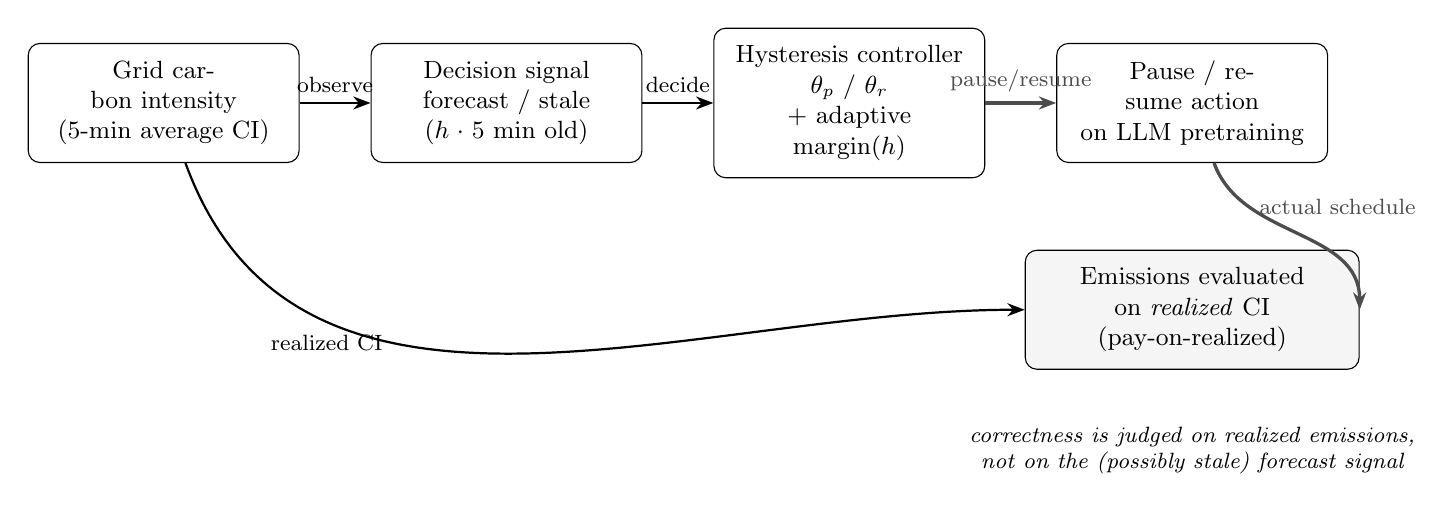
\begin{tikzpicture}[
    node distance=9mm,
    box/.style={draw, rounded corners=1.5mm, align=center, inner sep=2.2mm,
                text width=30mm, font=\small},
    evbox/.style={draw, rounded corners=1.5mm, align=center, inner sep=2.2mm,
                  text width=38mm, font=\small, fill=black!4},
    flow/.style={-{Stealth[length=2.2mm]}, thick},
    actflow/.style={-{Stealth[length=2.2mm]}, very thick, color=black!70},
  ]

  % --- main decision chain (decide on forecast) ---
  \node[box] (ci) at (0,0) {Grid carbon intensity\\ (5-min average CI)};
  \node[box, right=of ci] (sig) {Decision signal\\ forecast / stale\\ ($h \cdot 5$ min old)};
  \node[box, right=of sig] (hyst) {Hysteresis controller\\ $\theta_p$ / $\theta_r$\\ + adaptive margin($h$)};
  \node[box, right=of hyst] (train) {Pause / resume action\\ on LLM pretraining};

  \draw[flow] (ci) -- node[above, font=\footnotesize] {observe} (sig);
  \draw[flow] (sig) -- node[above, font=\footnotesize] {decide} (hyst);
  \draw[actflow] (hyst) -- node[above, font=\footnotesize] {pause/resume} (train);

  % --- pay-on-realized evaluation path ---
  \node[evbox, below=11mm of train] (eval) {Emissions evaluated\\ on \emph{realized} CI\\ (pay-on-realized)};

  \draw[flow] (ci) to[out=-70, in=180] node[left, font=\footnotesize, pos=0.35]
      {realized CI} (eval.west);
  \draw[actflow] (train) to[out=-70, in=90] node[right, font=\footnotesize, pos=0.25]
      {actual schedule} (eval.east);

  % --- annotation of the correctness loop ---
  \node[align=center, font=\footnotesize\itshape, below=6mm of eval]
    {correctness is judged on realized emissions,\\ not on the (possibly stale) forecast signal};
\end{tikzpicture}
\ifdefined\paperstandaloneinputsentinel
\else
\end{document}
\fi
}
  \caption{Decision pipeline. The controller decides on a forecast or stale
  signal ($h\cdot5$ minutes old) but pays on realized carbon intensity.}
  \label{fig:loop}
\end{figure}

\paragraph{Staleness model.}
A decision made on data that is $h$ 5-minute steps old is equivalent, for a
near-unit-root process, to a persistence forecast at horizon $h$. We formalize
both: a decision at staleness $h$ uses the AR(1) $h$-step-ahead forecast
$\hat{c}_t = \phi\, c_{t-h}$ (damped persistence, $\phi\approx1$), and the
\emph{empirical} $h$-step RMSE of that forecast is the decision-error scale we
measure.

\paragraph{Adaptive margin rule.}
{\sloppy To tolerate stale decisions, the controller widens the hysteresis margin
with $h$, using the AR(1) $h$-step prediction-interval scale: \par}
\begin{equation}
  \label{eq:margin}
  \mathrm{margin}(h) \;=\; c \cdot \sigma^* \cdot
    \sqrt{\frac{1-\phi^{2h}}{1-\phi^2}},
\end{equation}
with thresholds widened symmetrically around the optimized nominal midpoint,
$\theta_p(h) = \bar\theta + \mathrm{margin}(h)/2$ and
$\theta_r(h) = \bar\theta - \mathrm{margin}(h)/2$. $c=0$ recovers the nominal
thresholds; $\mathrm{margin}(0)=0$. At $\phi\approx1$ the scale factor grows
like $\sqrt{h}$, reaching $8.38\,\sigma^*\approx30.7$\,g/kWh at $h{=}72$ for
DE---the \emph{theoretical} AR(1) prediction-interval scale of the error a
six-hour-old decision faces; the empirical staleness error is about
$3.7\times$ larger (Section~\ref{sec:robustness}).

\paragraph{Metrics.}
Let $\mathcal{S}$ be the set of simulated training states under a policy, with
baseline = run the full job uninterruptedly at its start time. Savings
$S$ is the percentage of baseline carbon emissions avoided; overhead $O$ is the
wall-clock stretch (as a percentage of the uninterrupted makespan) caused by
pausing and checkpointing. A policy is \emph{within budget} if $O \le B$
(we use $B{=}200\%$) and \emph{completed} if the job finishes training inside
that budget. The optimizer maximizes $S$ subject to the budget (a savings
normalized score at $\alpha{=}1$); because the raw maximum score can select a
budget-blocked \emph{incomplete} run whose savings are inflated against a
full-run baseline, we always report the \emph{completed-feasible} optimum and,
when it matters, an explicit completion constraint. The \emph{grace horizon}
$g$ is the largest $h\in\{1,3,6,12,24,72\}$ with savings degradation
$\le 10\%$ relative to the fresh-decision policy.

\section{Grid Carbon Intensity at 5-minute Resolution}
\label{sec:grid}

\paragraph{Data.}
We use average carbon intensity (ACI) traces from Electricity Maps
\cite{electricitymaps}: five grids (DE, IT, SE, US, CN), years 2022--2026, at
5-minute resolution (105{,}120 points/year; 105{,}408 in the leap year 2024).
Experiments use the three regions
DE, IT, SE across 2022--2025 (2022--2024 train, 2025 test). ACI is the
location-based Scope-2 signal operators actually have; we return to the
average-vs-marginal and MCI questions in Section~\ref{sec:discussion}
\cite{sukprasert2024avm,wiesner2025beyondmci}.

\paragraph{CI is a near-unit-root process.}
At 5-minute resolution, grid CI is dominated by its own past. Table~\ref{tab:cal}
shows the fitted AR(1) parameters on 2022--2024: lag-1 autocorrelation
$\approx0.996$--$0.9997$, innovation standard deviation $\sigma^*$ of
$0.77$--$4.42$\,g/kWh. Figure~\ref{fig:trace} shows a 48-hour sample and the
year-long autocorrelation function: autocorrelation at lag 1 is $\approx0.9995$
(DE) and decays only slowly ($\approx0.72$ at 24\,h).

\begin{table}[t]
  \caption{AR(1) calibration (train 2022--2024, test 2025) and persistence
  vs.\ AR(1) evaluation RMSE. Max persistence--AR(1) gap across all horizons:
  $0.0512$\,g/kWh (IT, $h{=}72$).}
  \label{tab:cal}
  \small
  \begin{tabular}{@{}l c c c c c@{}}
    \toprule
    Region & $\phi$ & lag-1 & $\sigma^*$\,(g/kWh) & RMSE($h{=}1$) & RMSE($h{=}72$) \\
    \midrule
    DE & 0.9997 & 0.9997 & 3.66 & 4.21 & 113.4 \\
    IT & 0.9987 & 0.9987 & 4.42 & 5.02 & 77.6 \\
    SE & 0.9960 & 0.9960 & 0.77 & 0.78 & 7.8 \\
    \bottomrule
  \end{tabular}
\end{table}

\begin{figure}[t]
  \centering
  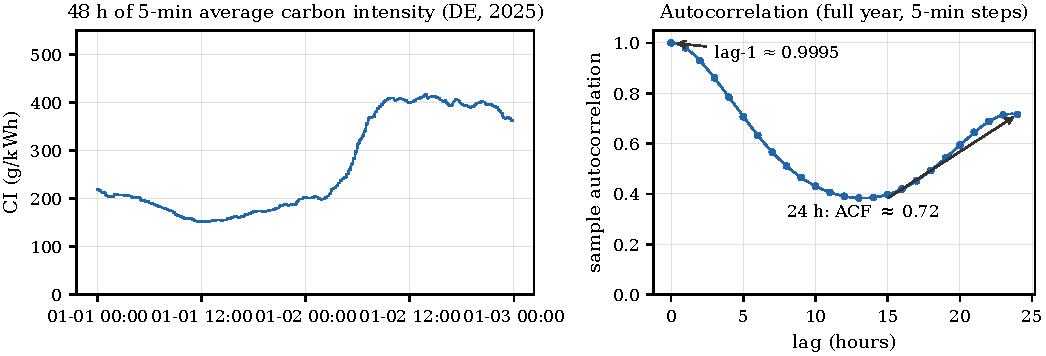
\includegraphics[width=\columnwidth]{figures/ci_trace_acf}
  \caption{Left: 48\,h of 5-minute DE 2025 CI. Right: sample autocorrelation to
  lag 288 (24\,h), annotated at lag-1 $\approx0.9995$ and 24\,h
  $\approx0.72$.}
  \label{fig:trace}
\end{figure}

\paragraph{Persistence $\approx$ AR(1) $\approx$ AR(7).}
At the decision scale, what matters is not which forecaster you use but how the
error grows with staleness. Figure~\ref{fig:rmse} shows evaluation RMSE versus
horizon for persistence, AR(1), and AR(7) on 2025. Persistence and AR(1) are
statistically indistinguishable at every horizon (max gap $0.0512$\,g/kWh at
IT, $h{=}72$, i.e.\ $\le0.06$). The richer AR(7) shaves at most a few g/kWh off
the short-horizon error (e.g.\ DE $h{=}1$: 2.3 vs.\ 4.2\,g/kWh) and converges
to the same error at $h\ge24$. On thresholds of order 18--270\,g/kWh, neither
difference is decision-relevant. The entire multi-day CI-forecasting program
\cite{maji2022dacf,maji2023carboncast,yan2025ensembleci,maji2025carbonx}
improves short-horizon forecast quality at hourly resolution; our measurement
shows that at the 5-minute pause/resume decision scale the error budget is
dominated by staleness, not by forecaster choice.

\begin{figure}[t]
  \centering
  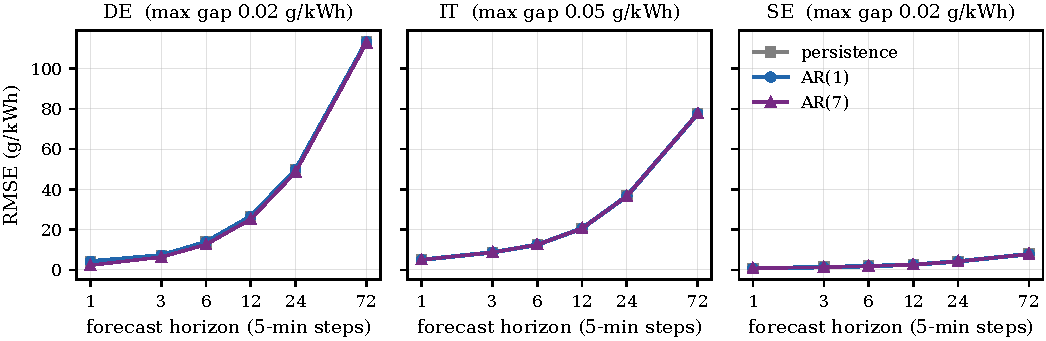
\includegraphics[width=\columnwidth]{figures/rmse_horizon}
  \caption{RMSE vs.\ horizon (log-x) for persistence, AR(1), AR(7); per region.
  Persistence--AR(1) gap $\le 0.06$\,g/kWh everywhere.}
  \label{fig:rmse}
\end{figure}

\section{Threshold Optimization \& Design Rules}
\label{sec:design}

\paragraph{Optimizer.}
We optimize $(\theta_p,\theta_r)$ with an adaptive grid search
(resolution 10, six iterations) over the DeepSeek profile, 2025 data, budget
200\%, $\alpha{=}1$, fixed per-region training start (DE 02-01, IT 01-14,
SE 04-22). The optimizer maximizes the savings-normalized score
$\mathrm{score}=\tfrac{1}{2}(\alpha\,S/100+1-(1-\alpha)\,O/B)$
under budget $B$; at $\alpha{=}1$ the overhead term vanishes
($\mathrm{score}=(S/100{+}1)/2$), so the budget binds only through the explicit
overhead constraint---the source of the budget-blocked runs guarded below. The baseline optima are
DE $(\theta_p,\theta_r)=(272.37,267.73)$, $S{=}43.35\%$, $O{=}174.3\%$;
IT $(246.70,230.45)$, $S{=}32.67\%$, $O{=}194.7\%$;
SE $(18.18,17.51)$, $S{=}23.17\%$, $O{=}106.3\%$.

\paragraph{Evaluation protocol.}
Every experiment shares one protocol: the job starts at a fixed date; the
policy observes a decision signal (forecast, stale realization, or biased
signal), pauses/resumes training accordingly, and emissions are accumulated on
the \emph{realized} 5-minute CI series. Savings $S$ is the percentage of
baseline carbon avoided, overhead $O$ the percentage wall-clock stretch, and the
optimizer selects the feasible point maximizing the savings-normalized score
at $\alpha{=}1$ under the overhead budget $B$. Because the raw max-score point
can be a budget-blocked \emph{incomplete} run, every reported optimum is the
completed-feasible one; when the two differ we report both and say so. All
pipelines are deterministic (no RNG in the optimizer or decision path), all
parameters are fixed in the committed configuration, and every figure in this
paper is generated from the committed JSON/CSV artifacts rather than recomputed
from scratch.

\paragraph{The optimized margin is near zero---and this is a property of the
signal, not the optimizer.}
The Pareto frontiers (Figure~\ref{fig:pareto}) show that a small hysteresis
margin achieves most achievable savings: DE margin 4.64, IT 16.25, SE 0.67
g/kWh. This is consistent with the theoretical result that double-threshold
policies are optimal \cite{lechowicz2023opr}: the margin is just large enough to
absorb checkpoint cost. The \emph{near-zero-margin} design rule holds across
years for SE (0.67--0.75\,g/kWh, all four years). For DE and IT the rule is
energy-crisis-sensitive: 2022--2023 push DE margins to 15--16\,g/kWh and IT's
2025 reopt operating point is 16.25\,g/kWh. We therefore state the rule as
\emph{margin scale}, not as a universal value.

\begin{figure}[t]
  \centering
  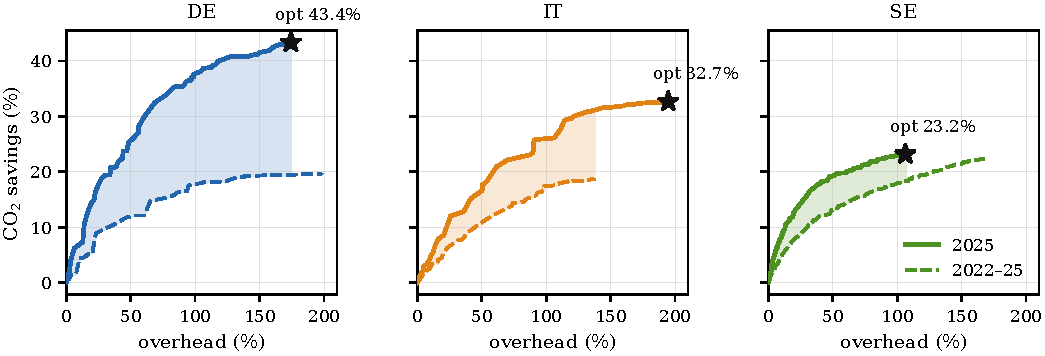
\includegraphics[width=\columnwidth]{figures/pareto}
  \caption{Pareto frontiers (overhead vs.\ savings), 2025 run (solid) with
  2022--2025 pooled envelope (shaded).}
  \label{fig:pareto}
\end{figure}

\paragraph{Percentile thresholds are not year-stable.}
The implied threshold percentiles wander by 11--15\,pp across years
(DE $\theta_p$ exceedance 59.9--71.2\%, IT 60.3--74.0\%, SE 60.0--74.8\%). We
deliberately do \emph{not} claim a universal threshold percentile. Likewise,
optimized \emph{savings} are year-specific (DE 14.95--43.35\%, IT 10.02--32.67\%,
SE 16.18--23.17\%): grids decarbonize and energy crises arrive, so the absolute
opportunity moves. Table~\ref{tab:rules} summarizes the rule-deviation audit
over 2022--2025.

\begin{table}[t]
  \caption{Multi-year design-rule audit (2022--2025; tolerances 10\,g/kWh
  margin, 10\,pp percentile, 1 grid step grace).}
  \label{tab:rules}
  \small
  \begin{tabular}{@{}l c c c@{}}
    \toprule
    Region & margins 22--25 (g/kWh) & S range (\%) & grace 23/24/25 \\
    \midrule
    DE & 16.00 / 15.04 / 4.76 / 4.64 & 14.95--43.35 & 24/24/24 \\
    IT & 3.24 / 8.00 / 4.72 / 16.25 & 10.02--32.67 & 72/24/12 \\
    SE & 0.75 / 0.67 / 0.72 / 0.67 & 16.18--23.17 & 12/12/12 \\
    \bottomrule
  \end{tabular}
\end{table}

\paragraph{The grace horizon is stable within regions---with a censored outlier.}
The grace horizon (maximum staleness with $\le 10\%$ savings loss) is 24/12/12
steps for DE/IT/SE in 2025. DE (24/24/24) and SE (12/12/12) are stable across all
three years; IT's 2024--25 horizons (24, 12) are within one grid step of each
other, but 2023 (72) is a right-censored outlier---2023 CI never crosses the
10\% degradation level even at $h{=}72$ (3.1\%), so the ``year-stable'' reading
for IT rests on two of three years with a documented exception. The absolute
savings \emph{levels} are not stable (7--28\,pp swings as grids decarbonize and
energy crises arrive), but the two \emph{structural} rules (margin scale, grace
horizon) hold as stated. Figure~\ref{fig:heatmap} shows the region-year savings
and margin surfaces.

\begin{figure}[t]
  \centering
  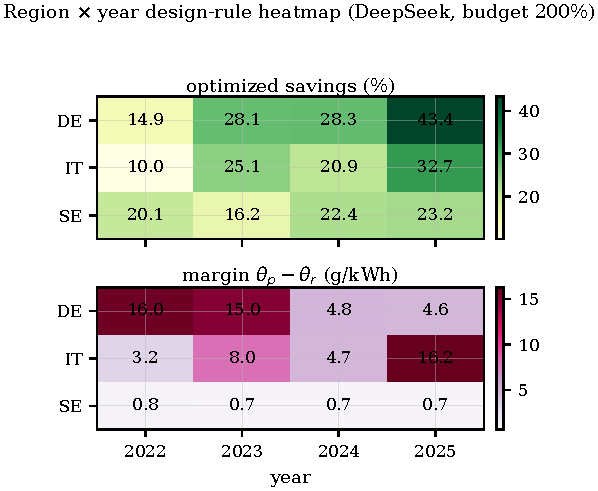
\includegraphics[width=\columnwidth]{figures/heatmap_year_region}
  \caption{Region $\times$ year optimized savings (top) and margins (bottom).
  Savings levels are year-specific; margin \emph{scale} is stable.}
  \label{fig:heatmap}
\end{figure}

\paragraph{Budget sweep: the frontier collapses only where the operating point
is already near the cap.}
\begin{table}[t]
  \caption{Overhead-budget sweep (2025, DeepSeek). Completed-feasible savings
  \% at each budget. IT's feasible frontier collapses at $B\le50\%$; DE and SE
  degrade gracefully.}
  \label{tab:budget}
  \small
  \begin{tabular}{@{}l c c c c c@{}}
    \toprule
    Region & $B{=}30$ & $B{=}50$ & $B{=}100$ & $B{=}200$ & collapse \\
    \midrule
    DE & 11.51 & 16.28 & 29.52 & 43.35 & -- \\
    IT & -- & -- & 19.85 & 32.67 & $B \le 50$\% \\
    SE & 14.59 & 18.36 & 22.87 & 23.17 & -- \\
    \bottomrule
  \end{tabular}
\end{table}
At budget $B{=}30\%$, DE and SE still find completed-feasible points
($S{=}11.51\%$ and $14.59\%$); IT finds \emph{none} at $B\le50\%$, because its
nominal operating point already sits at $194.7\%$ overhead. IT has no room to
tighten; its frontier collapses. These are completed-feasible values; the raw
max-score optimum can be an incomplete, budget-blocked run with inflated
savings (e.g.\ IT $B{=}100\%$: raw 82.00\% vs.\ completed-feasible 19.85\%).

\paragraph{Checkpoint realism: savings survive, the design rules change.}
\label{sec:ckpt}
Table~\ref{tab:ckpt} reports the checkpoint-realism sweep (the decisive Story-A
experiment). At 900\,s and 2700\,s full-state checkpoint/restore, the
completed-feasible optimum retains $97.6\%$, $94.6\%$, $95.2\%$ (at 900\,s) and
$91.4\%$, $85.3\%$, $81.4\%$ (at 2700\,s) of the 148.8\,s-savings for DE/IT/SE.
Two design rules change with checkpoint cost.
First, the optimized margin must widen (DE 4.64$\to$16.59 at 900\,s,
$\to$39.50 at 2700\,s); the margin absorbs the checkpoint cost, as the
checkpoint-cost-derived separation in DTPR predicts \cite{lechowicz2023opr}.
Second, an explicit completion constraint becomes required: at 900/2700\,s the
raw max-score optimum for DE/IT is an incomplete budget-blocked run whose
reported savings are inflated (DE 47.91\%$\to$82.18\%), so any deployment under
minutes-scale checkpoints must enforce completion, not raw score.

\begin{table}[t]
  \caption{Checkpoint-realism sweep (2025). Completed-feasible savings and
  retention vs.\ the 148.8\,s optimum.}
  \label{tab:ckpt}
  \footnotesize
  \begin{tabular}{@{}l c c c c c@{}}
    \toprule
    Region & $S_0$ (148.8\,s) & $S$(900\,s) & $S$(2700\,s) & $R$@900 & $R$@2700 \\
    \midrule
    DE & 43.35\% & 42.32\% & 39.60\% & 97.6\% & 91.4\% \\
    IT & 32.67\% & 30.90\% & 27.87\% & 94.6\% & 85.3\% \\
    SE & 23.17\% & 22.06\% & 18.87\% & 95.2\% & 81.4\% \\
    \bottomrule
  \end{tabular}
\end{table}

\section{Forecast Robustness: Noise vs.\ Staleness}
\label{sec:robustness}

\subsection{The decomposition}
\begin{figure}[t]
  \centering
  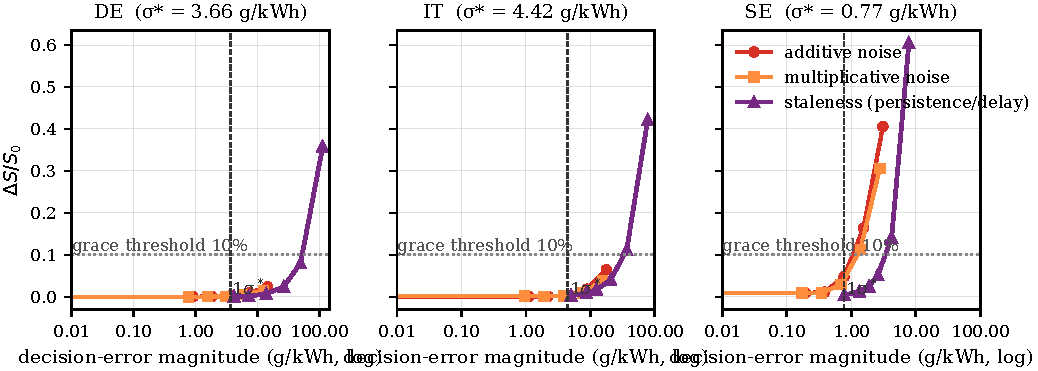
\includegraphics[width=\columnwidth]{figures/noise_vs_staleness}
  \caption{Savings degradation $\Delta S/S_0$ vs.\ decision-error magnitude for
  forecast \emph{noise} (additive/multiplicative, in $\sigma^*$ units) and
  decision \emph{staleness} (persistence RMSE at horizon $h$), on a shared
  g/kWh axis. Loss scales with error magnitude; at matched magnitude additive
  noise is the more damaging per unit error, while staleness is the failure mode
  that produces large errors ($h{=}72$ RMSE $\approx 7.8\times$ a $4\sigma^*$
  noise for DE).}
  \label{fig:noise}
\end{figure}
Figure~\ref{fig:noise} places the two error sources on one axis: the RMS
decision-error magnitude in g/kWh. Additive/multiplicative forecast noise at
level $\ell$ has magnitude $\ell\cdot\sigma^*$ (additive) or
$\ell\cdot\sigma_{rel}\cdot\mu$ (multiplicative); a stale decision at horizon
$h$ has magnitude equal to the persistence RMSE at $h$---a stale decision
\emph{is} a persistence forecast. Under the fixed (published) thresholds on
2025, a $4\sigma^*$ additive error costs $2.4\%$ (DE), $6.5\%$ (IT), and
$40.6\%$ (SE) of savings; a $1\sigma^*$ error costs $0.3\%$/$0.4\%$/$4.8\%$. SE's
fixed (published) policy uses the previously-published rounded thresholds
(19, 18), $s_0{=}22.87\%$, distinct from its 2025 reopt optimum
($18.18, 17.51 \rightarrow 23.17\%$); its margin (0.67\,g/kWh) is below its own
$\sigma^*$ (0.77), so noise is measured against a razor-thin band. The additive
family is tested only up to $4\sigma^*$; we do not extrapolate beyond it.

On the shared axis, at \emph{matched} error magnitude additive noise is
consistently the more damaging: DE, $4\sigma^*$ noise (14.6\,g/kWh) costs
$2.4\%$ vs.\ a 6-step-stale decision (13.9\,g/kWh) at $0.71\%$; IT, $6.5\%$
(17.7\,g/kWh) vs.\ $1.8\%$ (12.5\,g/kWh); SE, $40.6\%$ (3.1\,g/kWh) vs.\ $5.2\%$
(2.6\,g/kWh). White noise flaps the threshold; a smooth stale drift does not.
Staleness ``wins'' only through \emph{magnitude}: at $h{=}72$ the persistence
RMSE is $113.4$\,g/kWh (DE)---$7.8\times$ the $4\sigma^*$ noise (IT $77.7$ vs.\
$17.7$; SE $7.8$ vs.\ $3.1$)---and that error costs $35.8$/$42.2$/$60.5\%$
(DE/IT/SE; $2.4$/$4.1$/$5.2\%$ at 12 steps; grace 24/12/12). At the magnitudes
these modes realistically produce, a six-hour-stale decision costs $6$--$15\times$
more than a $4\sigma^*$ forecast error in DE and IT. This is the central
empirical result: \emph{decision-error magnitude dominates savings loss, and
staleness is the failure mode that generates large errors}.
Table~\ref{tab:degrad} reports the full grid.

\begin{table}[t]
  \caption{Fixed-policy (published thresholds) savings degradation
  $\Delta S/S_0$ (\%) on 2025. ``add $L$'' = additive error at
  $L\sigma^*$; ``pers $h$'' = persistence (stale) decision at horizon $h$.
  Multiplicative noise is strictly cheaper than additive (e.g.\ DE $1.5\%$
  at $4\sigma^*$).}
  \label{tab:degrad}
  \footnotesize
  \begin{tabular}{@{}l c c c c c c c c@{}}
    \toprule
    Region & add 1 & add 4 & pers 6 & pers 12 & pers 24 & pers 72 & grace \\
    \midrule
    DE & 0.3 & 2.4 & 0.7 & 2.4 & 8.0 & 35.8 & 24 \\
    IT & 0.4 & 6.5 & 1.8 & 4.1 & 11.2 & 42.2 & 12 \\
    SE & 4.8 & 40.6 & 2.5 & 5.2 & 14.2 & 60.5 & 12 \\
    \bottomrule
  \end{tabular}
\end{table}

\subsection{Reoptimizing thresholds under forecast bias}
Forecast \emph{bias} (not noise) is the regime where thresholds must move.
Reoptimizing thresholds under an additive bias of $1\sigma^*$/$2\sigma^*$ widens
the optimized margin from 4.64 to 16.68/28.36\,g/kWh (DE), 16.25 to
23.19/30.15\,g/kWh (IT), 0.67 to 3.21/5.49\,g/kWh (SE). The fixed margin rule
therefore does \emph{not} survive large additive bias in DE/IT (and fails for IT
even at delay-1: its margin stays at the 16.25 baseline while the decision
quality collapses); only SE's margin survives all tested bias levels. The correct
response to bias is reoptimization, not margin inflation; the correct response
to \emph{staleness} is the adaptive margin of Section~\ref{sec:adaptive}.
Figure~\ref{fig:drift} shows the threshold drift in the $(\theta_p,\theta_r)$
plane.

\begin{figure}[t]
  \centering
  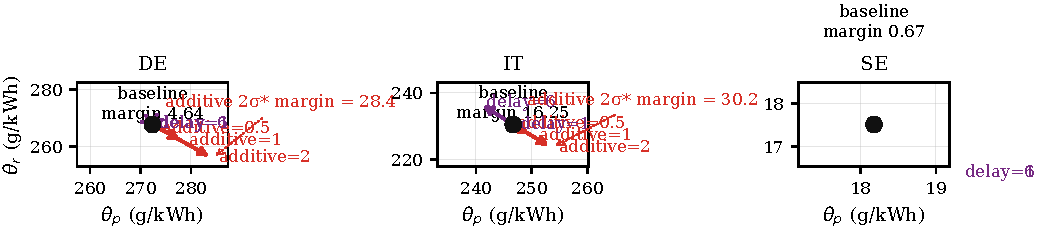
\includegraphics[width=\columnwidth]{figures/reopt_drift}
  \caption{Reoptimized threshold drift under additive forecast bias
  ($0.5/1/2\sigma^*$) and delay (1, 6 steps), per region. Margins widen
  substantially under bias (DE 4.64$\to$28.36\,g/kWh at $2\sigma^*$).}
  \label{fig:drift}
\end{figure}

\subsection{The grace horizon is predicted by the empirical AR(1) RMSE}
\begin{figure}[t]
  \centering
  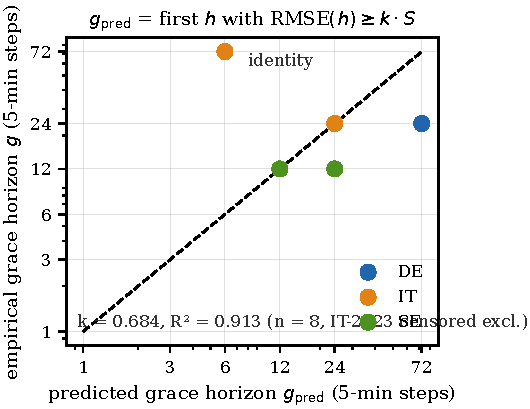
\includegraphics[width=\columnwidth]{figures/grace_horizon_map}
  \caption{Observed vs.\ predicted grace horizon (log-log). Prediction:
  empirical AR(1) RMSE($h$) crosses $k\cdot S$, $k{=}0.684$, $S{=}|\theta_p-\mu|$,
  $\mu$ = year-mean CI. $R^2{=}0.91$ on 8 region-years; IT-2023 (hollow) is a
  right-censored outlier.}
  \label{fig:grace}
\end{figure}
The grace horizon should be predicted, not just measured. Define
$S = |\theta_p - \mu|$, the distance from the pause threshold to the decision-year
mean CI ($\theta_p<\mu$ in all nine region-years, so the excursion sets the error
budget). We fit the hypothesis that the empirical
grace $g$ is the horizon where the empirical AR(1) $h$-step RMSE first reaches
$k\cdot S$. On 8 region-years (2023--2025, DE/IT/SE; IT-2023 excluded as a
right-censored outlier whose degradation never crosses 10\% even at $h{=}72$),
the through-origin fit gives $k{=}0.684$, a \emph{level-fit} $R^2{=}0.913$
(intercept fit $R^2{=}0.915$); 8/8 in-sample points lie within one grid step
(IT-2023, the excluded right-censored outlier, does not). Figure~\ref{fig:grace}
shows the map. Two caveats qualify this as a design rule rather than a
prediction method: the 8 region-years share only 4 distinct RMSE($g$) values
(DE 49.8\,g/kWh $\times$3, IT 36.6/20.6, SE 2.6\,g/kWh $\times$3) because the
RMSE($h$) curve is the 2025 calibration reused across years---so $R^2{=}0.91$ is
a \emph{level} fit RMSE($g$)$\approx k\cdot S$, not horizon-prediction
accuracy---and the horizon-space residuals are coarser (continuous residuals
$-7$ to $+8$ steps; DE-2024's grid prediction 72 vs.\ observed 24 is within one
grid step only on the coarse-grid metric, its continuous prediction being 29).
The usable output is the crossing rule $k\approx0.68$, not a horizon-level
predictor; this remains a \emph{conditional} headline---with IT-2023 included
the full-sample $R^2$ drops to 0.194, and the choice of $\mu$ matters (the
committed train-mean gives $R^2{=}0.86$, a near miss). If a reviewer rejects the censored
exclusion, the robust fallback reading is a design-rule observation: the grace
horizon sits where empirical RMSE $\approx 0.7\cdot S$.

Table~\ref{tab:gracepred} gives the per-region-year breakdown. The per-point
implied constants $k=\mathrm{RMSE}(g)/S$ are stable ($0.46$--$0.92$,
CV$\approx0.25$) without being universal---which is exactly the design-rule
regime we claim.

\begin{table}[t]
  \caption{Grace-horizon prediction, per region-year. $S=|\theta_p-\mu|$,
  $\mu$ = year-mean CI; $g_{pred}$ = smallest $h$ with empirical RMSE($h$)
  $\ge k\cdot S$, $k{=}0.684$. \textsuperscript{$\dagger$}right-censored outlier
  (excluded).}
  \label{tab:gracepred}
  \small
  \begin{tabular}{@{}l c c c c c@{}}
    \toprule
    region-year & $g$ & RMSE($g$) & $S$ & $g_{pred}$ & $g-g_{pred}$ \\
    \midrule
    DE-2023 & 24 & 49.8 & 59.4 & 24 & 0 \\
    DE-2024 & 24 & 49.8 & 89.0 & 72 & +1 step \\
    DE-2025 & 24 & 49.8 & 67.6 & 24 & 0 \\
    IT-2023$^\dagger$ & 72 & 77.6 & 16.3 & 6 & -- \\
    IT-2024 & 24 & 36.6 & 41.6 & 24 & 0 \\
    IT-2025 & 12 & 20.6 & 35.3 & 24 & +1 step \\
    SE-2023 & 12 & 2.6 & 5.6 & 24 & +1 step \\
    SE-2024 & 12 & 2.6 & 5.3 & 24 & +1 step \\
    SE-2025 & 12 & 2.6 & 2.8 & 12 & 0 \\
    \bottomrule
  \end{tabular}
\end{table}

\paragraph{Empirical, not theoretical, RMSE.}
The AR(1) \emph{theoretical} interval $\sigma^*\sqrt{(1-\phi^{2h})/(1-\phi^2)}$
systematically under-widens relative to the empirical evaluation RMSE---by up to
$3.7\times$ at $h{=}72$ for DE (30.7 vs.\ 113.4\,g/kWh), and the theoretical
crossing of $k\cdot S$ lies beyond the horizon grid for DE. The grace-horizon
prediction must therefore use the empirical RMSE curve; the model formula is
reported as a comparison and drives only the (conservative) adaptive margin of
Section~\ref{sec:adaptive}.

\section{Stale-Aware Adaptive Control}
\label{sec:adaptive}

\subsection{Controller}
Given the nominal optimized thresholds $(\bar\theta\pm \cdot)$ and a target
staleness $h$, the controller sets
$\mathrm{margin}(h)=c\cdot\sigma^*\cdot\sqrt{(1-\phi^{2h})/(1-\phi^2)}$
(Equation~\ref{eq:margin}) and widens symmetrically. $c$ is chosen on train
years 2022--2024 (per-region, by mean completion-guarded recovery over years
$\times$ horizons, ties to smaller $c$) and evaluated on 2025. Decisions use
the AR(1) $h$-step forecast; emissions use realized CI. We evaluate against
three baselines: \emph{naive-fixed} (published thresholds),
\emph{perfect-foresight} (identity decision), and a \emph{static oracle}
(per-$h$ reoptimized static thresholds). Two recovery metrics:
$\mathrm{recovery} =
\mathrm{clip}\big((S_{adapt}-S_{naive})/(S_{0}^{FF}-S_{naive}),\,0,\,1\big)$
(fraction of the naive-to-perfect loss closed) and
$\mathrm{recovery\_vs\_oracle} =
\mathrm{clip}\big((S_{adapt}-S_{naive})/(S_{oracle}-S_{naive}),\,0,\,1\big)$
(fraction of the \emph{recoverable}, naive-to-static-oracle gap closed). Both
are $0$ when the denominator is non-positive: $\mathrm{recovery}=0$ if
$S_{0}^{FF}\le S_{naive}$ (no positive loss to recover)---the SE case, whose
perfect-foresight baseline is the rounded-threshold control 22.87\%, below its
naive policy---and likewise
$\mathrm{recovery\_vs\_oracle}=0$ when $S_{oracle}\le S_{naive}$ (SE, all
$h\le12$). Because an incomplete run inflates savings, any incomplete row is
completion-guarded to zero; the guard changes only budget-exhausted rows---
every completed-run recovery is identical with or without it.

\begin{figure}[t]
  \centering
  \begin{minipage}{0.92\columnwidth}
  \small
  \begin{tabbing}
    \hspace{0.5em}\=\hspace{9em}\=\kill
    \textbf{Input:} nominal $(\theta_p^0,\theta_r^0)$, $\sigma^*$, $\phi$,\\
    \> grid $\mathcal{C}=\{0,0.25,0.5,0.75,1,1.5,2\}$\\
    \textbf{for} $c \in \mathcal{C}$ \textbf{do}\\
    \> $r[c] \gets$ mean completion-guarded recovery over\\
    \> \> train years $\times\, h \in \{1,3,6,12,24,72\}$\\
    \textbf{end for}\\
    $c^* \gets \arg\max_c r[c]$ (ties $\to$ smallest $c$)\\
    \textbf{at} staleness $h$:\\
    \> $m \gets c^*\sigma^*\sqrt{(1-\phi^{2h})/(1-\phi^2)}$\\
    \> $\theta_p \gets \bar\theta + m/2,\quad \theta_r \gets \bar\theta - m/2$\\
    \> \textbf{decide} on AR(1) $h$-step forecast, \textbf{pay} on realized CI
  \end{tabbing}
  \end{minipage}
  \caption{Stale-aware adaptive controller. $c^*$ selected on train years
  2022--2024; evaluated on 2025.}
  \label{fig:alg}
\end{figure}

\paragraph{Headline controller metric.}
$\mathrm{recovery}$ is dominated by the oracle-unreachable share of the loss;
$\mathrm{recovery\_vs\_oracle}$ is the informative measure of controller
quality. In absolute terms, the DE $h{=}1$ headline closes a recoverable gap of
only 0.07\,pp of savings (43.25$\to$43.32 vs.\ the 43.35 perfect-foresight
ceiling). Figure~\ref{fig:adaptive} and
Table~\ref{tab:adaptive} show the
closed loop at the train-selected $c^*$ (DE 0.75, IT 2, SE 1.5).

\begin{figure}[t]
  \centering
  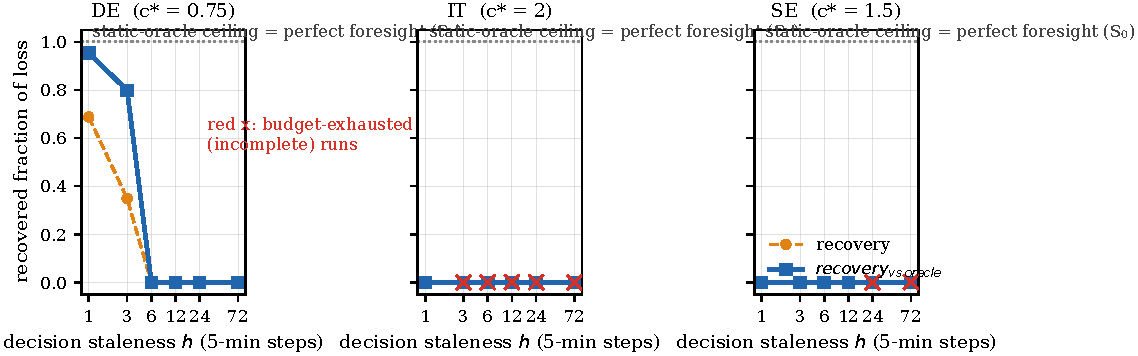
\includegraphics[width=\columnwidth]{figures/adaptive_recovery}
  \caption{Closed-loop recovery curves vs.\ staleness $h$. Solid:
  $\mathrm{recovery\_vs\_oracle}$ (headline); dashed: $\mathrm{recovery}$.
  Static-oracle ceiling = perfect foresight ($y{=}1$). Red $\times$:
  budget-exhausted (completion guard zeroes recovery).}
  \label{fig:adaptive}
\end{figure}

\begin{table}[t]
  \caption{Closed-loop results at the train-selected $c^*$ (test year 2025).
  DE $c^*{=}0.75$, IT $2$, SE $1.5$. $\mathrm{rvo}$ =
  $\mathrm{recovery\_vs\_oracle}$.}
  \label{tab:adaptive}
  \small
  \begin{tabular}{@{}l c c c c c c@{}}
    \toprule
    Region & $h$ & naive & adapt & oracle & recov. & rvo \\
    \midrule
    DE & 1 & 43.25 & 43.32 & 43.32 & 0.69 & \textbf{0.95} \\
    DE & 3 & 43.18 & 43.24 & 43.26 & 0.35 & \textbf{0.80} \\
    DE & 6 & 42.97 & 42.93 & 43.04 & 0.00 & 0.00 \\
    DE & 12 & 42.21 & 42.09 & 42.31 & 0.00 & 0.00 \\
    DE & 24 & 39.78 & 39.50 & 39.91 & 0.00 & 0.00 \\
    DE & 72 & 27.73 & 27.32 & 32.67 & 0.00 & 0.00 \\
    IT & 1 & 32.51 & 32.26 & 32.56 & 0.00 & 0.00 \\
    IT & 3 & 32.31 & \multicolumn{1}{c}{\emph{inc.}} & 32.35 & 0.00 & 0.00 \\
    IT & 6 & 32.05 & \emph{inc.} & 32.13 & 0.00 & 0.00 \\
    IT & 12 & 31.31 & \emph{inc.} & 31.44 & 0.00 & 0.00 \\
    IT & 24 & 28.96 & \emph{inc.} & 29.32 & 0.00 & 0.00 \\
    IT & 72 & 18.78 & \emph{inc.} & 25.50 & 0.00 & 0.00 \\
    SE & 1 & 23.09 & 21.98 & 23.09 & 0.00 & 0.00 \\
    SE & 3 & 22.92 & 21.70 & 22.92 & 0.00 & 0.00 \\
    SE & 6 & 22.68 & 21.32 & 22.68 & 0.00 & 0.00 \\
    SE & 12 & 22.17 & 17.87 & 22.17 & 0.00 & 0.00 \\
    SE & 24 & 20.23 & \emph{inc.} & 20.31 & 0.00 & 0.00 \\
    SE & 72 & 8.64 & \emph{inc.} & 12.93 & 0.00 & 0.00 \\
    \bottomrule
  \end{tabular}
\end{table}

\subsection{Calibrated claims}
The controller \emph{recovers most of the recoverable loss within the grace
region}: in DE it closes 95\% and 80\% of the naive-to-oracle gap at $h{=}1$ and
$h{=}3$ ($\mathrm{recovery\_vs\_oracle}=0.95/0.80$), i.e.\ it is near-optimal
exactly where staleness is small enough that the oracle itself can still help.
We do \emph{not} claim it recovers most of the total loss at large $h$; the
h=72 residual decomposes into three distinct shares:

Table~\ref{tab:csel} shows why $c^*$ selection is fragile. The train-year mean
recovery is near zero at every $c$ for all three regions ($\le0.056$); DE's
$c^*{=}0.75$ and IT's $c^*{=}2$ are each driven by a single 2024 cell, and 2022
contributes zero recovery in every region, while 2023 contributes zero for DE/IT
and $\le0.018$ for SE. The train-year signal simply
cannot discriminate among margins, which is itself a finding.

\begin{table}[t]
  \caption{Train-year (2022--2024) mean completion-guarded recovery by $c$;
  $c^*$ applied on 2025. The signal is near-zero and noisy.}
  \label{tab:csel}
  \small
  \begin{tabular}{@{}l c c c c c c c c@{}}
    \toprule
    Region & $c{=}0$ & 0.25 & 0.5 & 0.75 & 1 & 1.5 & 2 & $c^*$ \\
    \midrule
    DE & 0.006 & 0.006 & 0.017 & \textbf{0.056} & 0.012 & 0.000 & 0.016 & 0.75 \\
    IT & 0.004 & 0.003 & 0.000 & 0.000 & 0.002 & 0.010 & \textbf{0.025} & 2 \\
    SE & 0.000 & 0.002 & 0.022 & 0.016 & 0.022 & \textbf{0.029} & 0.000 & 1.5 \\
    \bottomrule
  \end{tabular}
\end{table}

\textbf{(a) Static-threshold-structural.} Even the \emph{static oracle}---per-$h$
reoptimized thresholds---recovers only 32\%/48\%/30\% of the h=72 loss
(DE/IT/SE): no static-threshold policy can do better, because a six-hour-stale
binary decision is simply too noisy.

\textbf{(b) Budget-bound.} IT's operating point sits at 194.7\% overhead; any
material margin widening is budget-infeasible (overhead hits 200\%, the run
stops incomplete). SE is budget-bound at $h\ge24$ at the train-selected
$c^*{=}1.5$. Widening ``recovers'' savings only by exhausting the budget and not
completing---the same inflation artifact documented in Section~\ref{sec:ckpt}.

\textbf{(c) $c$-selection fragility.} The margin rule is linear in $c$, so it
\emph{can} express the oracle scale: on DE $h{=}72$, $c{=}6$ reaches
$S{=}31.43\%$ (completed; $\mathrm{recovery\_vs\_oracle}{=}0.748$, near the
oracle's 32.67\%), and $c{=}8$ would reach 36.29\% but is budget-infeasible. Yet
the train-year signal cannot find that $c$ (Table~\ref{tab:csel}): the
$c$-grid ceiling is 2, so the deployed $c^*$ is far from the $c{\approx}6$ that
would approach
the oracle. The feasible-$c$ envelope corroborates: DE completes through
$c{=}6$ at $h{=}72$; IT's train-selected $c^*{=}2$ widening is budget-infeasible
at $h\ge3$, and most of IT's $c$-grid from $h{=}6$; SE completes only through $c{=}0.75$ at $h{=}72$
and no feasible $c$ recovers SE $h{=}72$ at all. Two further rule limitations
are documented: at $c{\approx}1$ the model interval under-widens relative to the
empirical staleness error ($3.7\times$ at $h{=}72$, DE), and symmetric widening
cannot express the oracle's $h{=}72$ center drift (DE oracle center
$\approx283$ vs.\ nominal midpoint 270.1\,g/kWh).

\subsection{DTPR comparison}
We benchmark a DTPR-style double-threshold policy with constant separation
$2\beta$, where $\beta$ is derived from the checkpoint/restore cycle's CO$_2$
cost ($\beta = (\tau_{pause}+\tau_{resume})/3600 \cdot \theta_p^{nominal}$:
11.26 / 10.20 / 0.75\,g/kWh for DE/IT/SE), operating on hourly-aggregated
signals \cite{lechowicz2023opr}. On the test year, the fixed-separation policy
is approximately neutral for DE/SE (savings within 1\,pp of the naive policy at
every horizon) and completion-infeasible for IT at every horizon
(budget-exhausted; its above-perfect reported savings are an incompleteness
artifact). The lesson:
constant margins derived from switching cost carry no completion-safety check,
whereas the adaptive rule's $c$-selection (with the completion guard) chooses
margins that complete where possible---the concrete way DTPR theory is extended
for frontier pretraining.

\paragraph{Design-rule outputs.}
Three rules follow: (i) under an overhead budget, budget headroom is a
prerequisite for adaptive widening---IT at $B{=}200\%$ has none; (ii) the
grace horizon is the operating point where an adaptive margin starts to matter,
and inside it the static oracle is nearly tight; (iii) the completion
constraint is first-class in both threshold design (Section~\ref{sec:ckpt}) and
adaptive margin selection.

\section{Discussion}
\label{sec:discussion}

\paragraph{Demand-side flexibility framing.}
We evaluate a \emph{single-site} workload; the grid-level value is that a
datacenter becomes a schedulable, flexible load rather than rigid demand
\cite{lin2023adapting,lin2024explodingai}. Hysteresis dead-bands are the
standard mechanism for this in demand response \cite{perfumo2011tcl}, and our
contribution is to make the dead-band \emph{stale-aware}.

\paragraph{Why 5-minute resolution matters.}
The whole CI-forecasting literature operates at hourly granularity
\cite{maji2022dacf,maji2023carboncast,yan2025ensembleci,maji2025carbonx}, and at
that granularity a single decision spans the entire dead-band. At 5-minute
resolution, by contrast, CI moves almost continuously (near-unit-root), so the
\emph{frequency} of decision-making is high enough that hysteresis and staleness
become the first-order effects---and it is precisely where they are that our
decomposition lives. A coarser (hourly) controller cannot exploit the brief
low-CI windows that the near-unit-root dynamics create, and it pays the
staleness cost of its own 12$\times$ coarser updates. The grace horizon is the
quantitative bridge between the two scales.

\paragraph{Aggregation and feedback effects.}
We analyze one operator. If many operators use the same signal and the same
grace horizon, their pause/resume actions will be correlated---precisely the
aggregation effect the equilibrium analysis warns about
\cite{jiang2026equilibrium}. Two mitigations follow from our results: first,
hysteresis margins (even near-zero ones) decorrelate the \emph{timing} of
switches, and the budget constraint binds each operator to a completed-feasible
regime; second, the demand-side-flexibility framing treats the schedule as a
curtailable, price-flexible load rather than a forecast follower. The design
rules here say nothing about system-level welfare; they say what a single
operator should do with the signal it has. Extending the analysis to
multi-operator equilibrium with explicit staleness is future work.

\paragraph{Signal choice: ACI, MCI, or excess power.}
Our traces are average carbon intensity (ACI), the location-based Scope-2
signal operators can actually obtain \cite{electricitymaps}. Moving-Beyond-MCI
argues marginal CI is non-observable and model-dependent (the provider
discontinued it), promoting \emph{excess power} as the actionable signal
\cite{wiesner2025beyondmci}; average-vs-marginal shows ACI-optimal and
MCI-optimal schedules can diverge \cite{sukprasert2024avm}; Green Mirage and
the attribution literature warn that location- vs.\ market-based estimates and
PPA accounting can mislead optimization \cite{maji2024greenmirage,
maji2024untangling}. Our framework is \emph{signal-agnostic}: the grace
horizon and adaptive margin are defined over the empirical $h$-step RMSE of
\emph{whatever} thresholded time series the operator uses, so the design rules
transfer to excess-power or MCI signals. We evaluate on realized emissions,
not on the signal, which is the property the equilibrium critique demands
\cite{jiang2026equilibrium}.

\paragraph{Equilibrium critique.}
The equilibrium analysis shows that average-CI-driven shifting can fail to
reduce system emissions when many agents react to the same a-posteriori signal
\cite{jiang2026equilibrium}. Our responses: (i) we \emph{pay on realized}
emissions, so savings claims are not conditional on the signal being causal;
(ii) we frame the work as demand-side flexibility provision, not as a claim
about market clearing; (iii) the grace-horizon/adaptive-margin machinery is
exactly a prescription for operating under the imperfect, possibly stale,
signals that current practice provides. The paper is best read as: \emph{given
the signal operators actually have, what is the least-bad control, and how much
does staleness cost?}

\paragraph{Average-vs-marginal accounting.}
Using ACI means our ``savings'' are Scope-2 (location-based average) savings,
not system-level emission reductions \cite{sukprasert2024avm}. We report this
honestly; the decision-theoretic structure (staleness decomposition, grace
horizon) is independent of the accounting basis.

\paragraph{When does noise start to matter?}
The low cost of additive noise is a \emph{measured} boundary condition, not a
law: it
holds when the optimized margin exceeds the noise scale. SE, whose margin
(0.67\,g/kWh) is \emph{below} its own $\sigma^*$ (0.77), degrades by 40.6\% at
$4\sigma^*$---noise matters whenever the signal-to-noise ratio of the
threshold band is unfavourable. The adaptive margin of
Section~\ref{sec:adaptive} is exactly the mechanism that restores that ratio
under staleness; the boundary condition also clarifies where ML forecasting
\emph{would} help (short-horizon, sub-margin error regimes) versus where it
cannot (staleness-dominated regimes). Operators in low-$\sigma^*$, low-margin
grids should treat forecast quality as first-class; those with material margins
(DE, IT) should spend their budget on signal freshness instead.

\paragraph{Embodied carbon and water.}
Operational carbon is a minority share of the full lifecycle for frontier
hardware, and the share is shrinking as hardware production amortizes across
fewer runs \cite{schneider2025lifecycle,luccioni2022bloom}; LLM-scale storage
embodied cost is also material \cite{tian2025greencache}. Temporal shifting
does not reduce embodied carbon (the GPUs are bought either way), but it does
not increase it either, and grid-flexible operation can reduce capacity
procurement if the grid rewards flexibility \cite{acun2023carbonexplorer}. Water
and other local impacts are out of scope.

\paragraph{Checkpoint realism.}
Minutes-scale checkpoints retain 81--97\% of savings (Section~\ref{sec:ckpt});
the checkpoint cost is real but not disqualifying. The dominant cost is not the
checkpoint \emph{time} but the overhead budget headroom it consumes, which is
why the completion constraint is a required design rule. For comparison,
suspend-resume alternatives that avoid checkpoint state (elastic scaling
\cite{hanafy2023carbonscaler}) are complementary levers, as are spatial
shifting \cite{bian2024cafe,gsteiger2024caribou}, carbon-aware LLM-inference
provisioning \cite{ecoserve2025}, and curtailment-driven
scheduling \cite{wiesner2026curtailment,wiesner2024fedzero}; single-site
temporal shifting bounds (EuroSys) \cite{sukprasert2024limitations} bound the
whole class.

\paragraph{A data-freshness SLA for operators.}
The grace horizon is directly deployable as a monitoring SLA: \emph{keep the
decision signal fresher than $g$ steps}. For DE that is 24 steps (2\,h), for
IT/SE 12 steps (1\,h); the operator can now budget for data-pipeline latency
and failover accordingly, and can sanity-check the target with the
$k{\approx}0.68\cdot S$ rule rather than trusting an ML forecaster whose error
is second-order. This is the practical counterpart to the UQ-Advice line: where
they spend effort quantifying forecast uncertainty \cite{johnson2025uqadvice},
we show the uncertainty that matters is the age of the signal.

\paragraph{Limitations.}
(1) The grace-horizon prediction depends on the choice of $\mu$ (year-mean CI
$R^2{=}0.91$; committed train-mean $R^2{=}0.86$) and on excluding IT-2023, a
right-censored outlier whose exclusion is load-bearing for the $R^2$.
(2) The
adaptive rule widens symmetrically and cannot express the oracle's center
drift at large $h$. (3) We study single-site operation in three regions; US/CN
traces are available but unused here. (4) The low measured cost of additive
noise holds where the optimized margin exceeds the noise scale (DE, IT) and only
within the tested $4\sigma^*$ range; SE's sub-$\sigma^*$
margin is noise-sensitive. (5) Our savings are Scope-2 average-CI savings, not
attributed system-level reductions \cite{sukprasert2024avm,jiang2026equilibrium}.

\section{Conclusion}
\label{sec:conclusion}
At the 5-minute decision scale, decision-error \emph{magnitude} dominates the
savings lost to carbon-aware pause/resume in frontier LLM pretraining: the
failure mode that generates large errors is decision \emph{staleness}, not
forecast \emph{noise}---near-unit-root drift makes a six-hour-old decision a
$113.4$\,g/kWh error (DE), $7.8\times$ a $4\sigma^*$ forecast error, costing
35.8--60.5\% of savings versus $<$7\% for the $4\sigma^*$ noise in DE and IT; at
\emph{matched} magnitude additive noise is the more damaging per unit error, so
the lever is signal freshness, not forecast accuracy. We
characterized 5-minute grid CI as near-unit-root, introduced the grace horizon
as the maximum staleness with $\le10\%$ loss and predicted it from the empirical
AR(1) RMSE ($k{\approx}0.68\cdot S$, level-fit $R^2{=}0.91$), and showed that a
stale-aware adaptive hysteresis controller closes 95\%/80\% of the recoverable
naive-to-oracle gap at one/three decision steps, with the large-$h$ residual
honestly split into static-threshold-structural, budget-bound, and
$c$-selection-fragile shares. Under minutes-scale checkpoints for a 671B-model,
completed-feasible retention is 81--97\%, at the price of a wider margin and an
explicit completion constraint. The takeaway is a forecast-agnostic design kit:
near-zero margin scale, a grace horizon stable in normal years (IT-2023 a
documented outlier), and a data-freshness SLA.\looseness=-1

\bibliographystyle{ACM-Reference-Format}
\bibliography{references}

\end{document}
